\documentclass{beamer}
\usepackage[utf8]{inputenc}
\usepackage[francais]{babel}

\usepackage{tabularx}
\usepackage{subfig}
\usepackage{listings}
\usepackage{verbatim}

\usetheme{Atilla}
\usecolortheme{atilla1}

\author{Pierre Sudron}
\title{{\huge git pour les novices}}
\institute{EISTI}
\date{\today}

\begin{document}

\begin{frame}[t,plain]
\titlepage
\end{frame}

\begin{frame}{git est un système de gestion de sources}
	\begin{itemize}
		\item gérer l'évolution d'un code
		\item partager efficacement son travail en équipe
		\item garder un historique de l'évolution d'un projet
		\item travailler en parallèle
	\end{itemize}
	\begin{center}
		
\includegraphics[width=3cm]{img/search}
	\end{center}
\end{frame}

\begin{frame}{autres systèmes existants}
	\begin{itemize}
		\item Subversion (svn)
		\item Mercurial (Hg)
		\item Bazaar (bzr)
		\item autres systèmes propriétaires
	\end{itemize}
\end{frame}

\begin{frame}{Plus particulièrement sur git}
	\begin{itemize}
		\item créé pour le noyau Linux
		\item développé par Junio Hamano
		\item distribué et très flexible
		\item adoption rapide et massive depuis 2005
	\end{itemize}
	
	\begin{center}
		
\includegraphics[height=2cm]{img/Git-logo}
	\end{center}	
\end{frame}


\begin{frame}{Qu'est-ce que git peut m'apporter ?}
	\begin{itemize}
		\item suivi précis de l'avancement d'un projet
		\item souplesse dans l'évolution
		\item facilité de mise en commun
	\end{itemize}
\end{frame}

\begin{frame}{Intégration douloureuse : un projet qui fait plouf}
	\begin{center}
		
\includegraphics[height=4cm]{img/bob_bob}\\
		\Large{Bob et Bob travaillent sur un projet\\et se répartissent les t\^aches}
	\end{center}
\end{frame}

\begin{frame}{À deux jours du livrable...}
	\begin{center}
		
\includegraphics[height=4cm]{img/bob1}\\
		\Large{Bob a bien avancé sur sa partie}
	\end{center}
\end{frame}

\begin{frame}
	\begin{center}
		
\includegraphics[height=5cm]{img/bob2}\\
		\Large{Bob pas tellement\\mais il a fait quelque chose au moins}
	\end{center}
\end{frame}

\begin{frame}{C'est l'heure de mettre en commun !}
	\begin{center}
		
\includegraphics[height=4cm]{img/bob_bob2}\\
		\Large{Et quelle surprise, ça marche pas !}
	\end{center}
\end{frame}

\begin{frame}
	\begin{center}
		
\includegraphics[height=5cm]{img/bobracha}\\
		\Large{Et à 24 heures du rendu, c'est un peu cuit...}
	\end{center}
\end{frame}

\begin{frame}{L'intégration progressive}
	\begin{itemize}
		\item git incite à mettre en commun très régulièrement
		\item en cas d'ennui, il est possible de revenir à la dernière version fonctionnelle
		\item de là, il est facile de voir les modifications ultérieures et isoler le code en cause
	\end{itemize}
	\begin{center}
		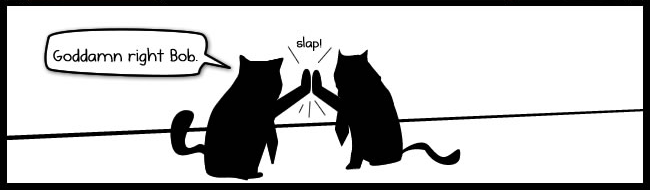
\includegraphics[height=2cm]{img/ok_bob}
	\end{center}
\end{frame}

\begin{frame}{De quoi ai-je besoin ?}
	\begin{center}
 		\Large{Rien}\\
 		{\small  \textit{(mais sous Linux, hein...)}}
	\end{center}

	\begin{figure}
		\centering
		
\includegraphics[height=3cm]{img/terminal}
	\end{figure}
\end{frame}

\begin{frame}{Principes de fonctionnement}

	En \textbf{local}, on travaille avec 3 éléments :
	\begin{figure}
  		\centering
 		\subfloat{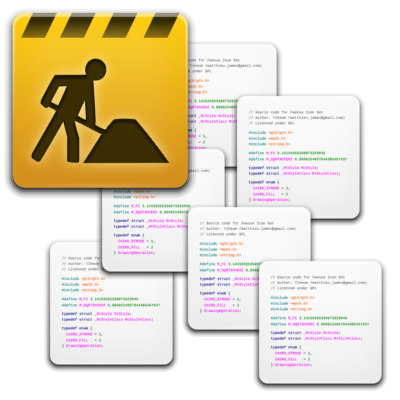
\includegraphics[width=2cm]{img/working_dir}}     
		\subfloat{
\includegraphics[width=1.5cm]{img/forward}}
  		\subfloat{
\includegraphics[width=2cm]{img/stash}}
  		\subfloat{
\includegraphics[width=1.5cm]{img/forward}}
  		\subfloat{
\includegraphics[width=2cm]{img/git_repo}}
	\end{figure}
	
	\begin{center}
		\begin{tabular}{p{2cm} p{0.7cm} p{2cm} p{0.7cm} p{2cm}}
		\centering dossier de travail & & \centering fichiers indexés & & \centering dépôt local
		\end{tabular}
	\end{center}
\end{frame}

\begin{frame}{Contenu d'un dépôt git}
	\begin{center}
		Succession de \textbf{commits}\\
	\end{center}
	\begin{figure}
		\centering
		
\includegraphics[height=2.5cm]{img/repo1}
	\end{figure}
	Un commit est un jeu de modifications, c'est l'\textit{atome} de git.
\end{frame}


\begin{frame}{Mise en commun}
	\begin{center}
		Synchronisation entre le dépôt local et un dépôt distant
	\end{center}
	
	\begin{figure}
  		\centering
 		\subfloat{
\includegraphics[height=3cm]{img/git_repo}}     
		\subfloat{
\includegraphics[height=2.5cm]{img/sync}}
  		\subfloat{
\includegraphics[height=3cm]{img/web}}
	\end{figure}
\end{frame}

\begin{frame}
	\begin{center}
 		\Large{Partie 1 : C'est un voyage qu'il faut commencer seul}\\
 		{\small  \textit{versionnage d'un simple fichier texte}}
	\end{center}

	\begin{figure}
		\centering
		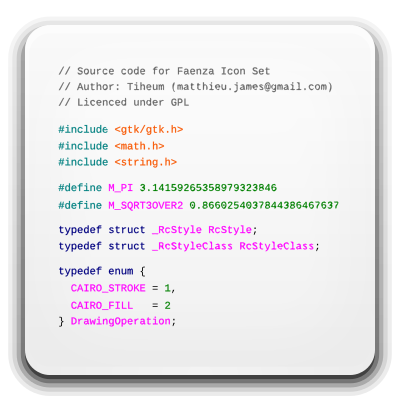
\includegraphics[height=3cm]{img/source}
	\end{figure}
\end{frame}

\begin{frame}[fragile]{Configuration de git : qui suis-je ?}
	git retrace l'évolution du projet ainsi :
	\begin{center}
		\textbf{qui} a fait \textbf{quoi}, et \textbf{quand}
	\end{center}
	
	Pour définir \textbf{qui} est l'utilisateur :
	\begin{lstlisting}[frame=single]
		git config --global user.name "Votre nom"
		git config --global user.email "root@atilla.org"
	\end{lstlisting}

\end{frame}

\begin{frame}[fragile]{Préparer le projet}
	Se placer dans le dossier de travail (le créer si besoin) :
	\begin{lstlisting}[frame=single]
		mkdir ~/formation_git
		cd ~/formation_git/
	\end{lstlisting}
	
	Initialiser git dans ce répertoire :
	\begin{lstlisting}[frame=single]
		git init
	\end{lstlisting}
\end{frame}

\begin{frame}{Comment ça se présente}
\begin{center}
	\begin{tabular}{l c l}
	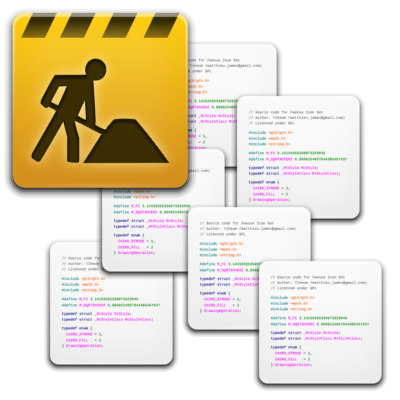
\includegraphics[width=1cm]{img/working_dir} & \textbf{répertoire de travail :} & vide \\
	
\includegraphics[width=1cm]{img/stash} & \textbf{fichiers indexés :} & vide \\
	
\includegraphics[width=1cm]{img/git_repo} & \textbf{dépôt local :} & initialisé et vide \\ 
	\end{tabular} 
\end{center}
\end{frame}

\begin{frame}[fragile]{Créer un fichier}
	Sans changer de dossier, créer un fichier \textbf{README} avec le contenu suivant :
	\begin{lstlisting}[frame=single]
		Formation git
	\end{lstlisting}
	Enregistrer le fichier
\end{frame}

\begin{frame}{Comment ça se présente}
\begin{center}
	\begin{tabular}{l c l}
	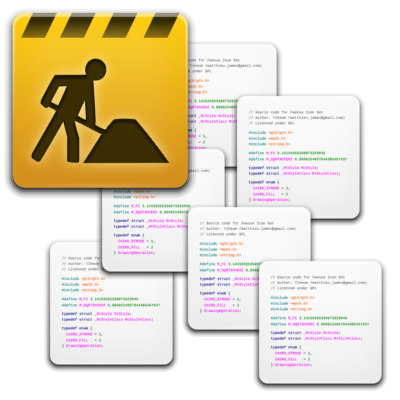
\includegraphics[width=1cm]{img/working_dir} & \textbf{répertoire de travail :} & README \\
	
\includegraphics[width=1cm]{img/stash} & \textbf{fichiers indexés :} & vide \\
	
\includegraphics[width=1cm]{img/git_repo} & \textbf{dépôt local :} & initialisé et vide \\ 
	\end{tabular} 
\end{center}
\end{frame}

\begin{frame}[fragile]{Constater les changements avec git status}
	\begin{lstlisting}[frame=single]
		git status
	\end{lstlisting}
	\begin{figure}
		\centering
		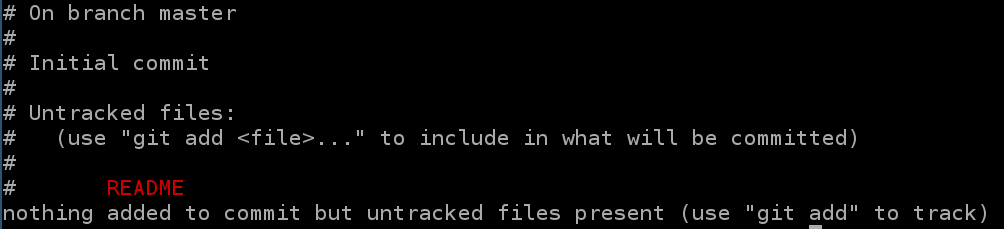
\includegraphics[width=11.5cm]{img/shot1}
	\end{figure}
	\begin{center}
	\textit{README n'est pas indexé}, on nous propose d'utiliser git add
	\end{center}
\end{frame}

\begin{frame}[fragile]{Indexer un fichier avec git add}
	\begin{lstlisting}[frame=single]
		git add README
	\end{lstlisting}
	
	\begin{figure}
  		\centering
 		\subfloat{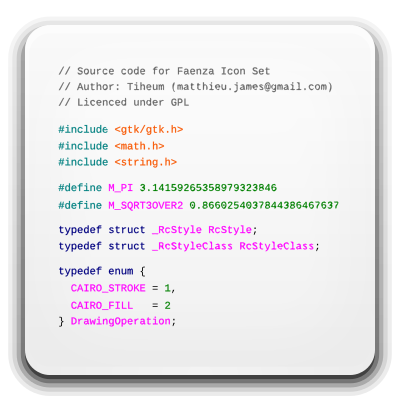
\includegraphics[height=2.5cm]{img/source}}     
		\subfloat{
\includegraphics[height=2cm]{img/forward}}
  		\subfloat{
\includegraphics[height=3.5cm]{img/stash}}
	\end{figure}
\end{frame}

\begin{frame}{Comment ça se présente}
\begin{center}
	\begin{tabular}{l c l}
	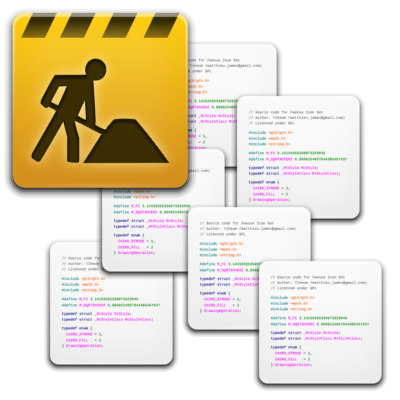
\includegraphics[width=1cm]{img/working_dir} & \textbf{répertoire de travail :} & README \\
	
\includegraphics[width=1cm]{img/stash} & \textbf{fichiers indexés :} & README (nouveau fichier)\\
	
\includegraphics[width=1cm]{img/git_repo} & \textbf{dépôt local :} & initialisé et vide \\ 
	\end{tabular} 
\end{center}
\end{frame}

\begin{frame}[fragile]{Constater les changements avec git status}
	\begin{lstlisting}[frame=single]
		git status
	\end{lstlisting}
	\begin{figure}
		\centering
		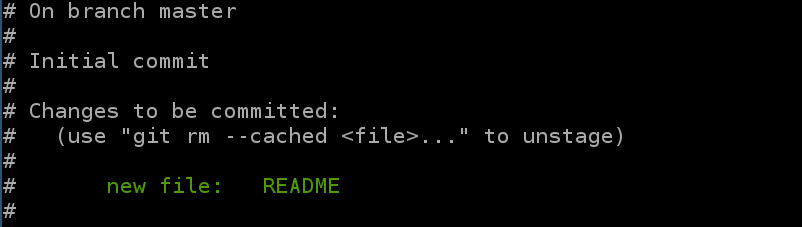
\includegraphics[width=11.5cm]{img/shot2}
	\end{figure}
	\begin{center}
	\textit{README est dans l'index} en tant que nouveau fichier
	\end{center}
\end{frame}

\begin{frame}[fragile]{Notre premier git commit}
	On va mettre à jour le dépôt local et laisser une trace de la création du fichier README
	\begin{lstlisting}[frame=single]
		git commit -m "Ajout du fichier README"
	\end{lstlisting}
	
	Tout commit est décrit par un \textbf{message}, il doit être :
		\begin{itemize}
		\item \textbf{précis}
		\item \textbf{concis}
		\end{itemize}	
\end{frame}

\begin{frame}{Comment ça se présente}
	\begin{center}
		\begin{tabular}{l c l}
		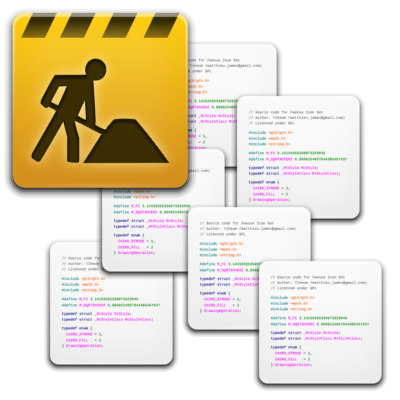
\includegraphics[width=1cm]{img/working_dir} & \textbf{répertoire de travail :} & README \\
		
\includegraphics[width=1cm]{img/stash} & \textbf{fichiers indexés :} & \textbf{vide}\\
		
\includegraphics[width=1cm]{img/git_repo} & \textbf{dépôt local :} & commit \texttt{abcdef01} (no1) \\ 
		\end{tabular} 
	\end{center}

	\begin{center}
		\textit{(vérifier avec git status)}
	\end{center}
\end{frame}

\begin{frame}{Historique des commits}

	\begin{figure}
		\centering
		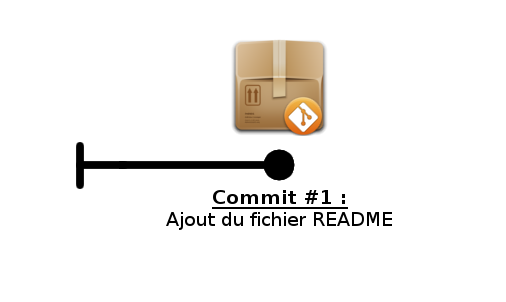
\includegraphics[height=5cm]{img/repo2}
	\end{figure}
\end{frame}

\begin{frame}[fragile]{Poursuivons le travail...}

	Ajouter une ligne à la fin du fichier \textbf{README} :
	\begin{lstlisting}[frame=single]
		Formation git
		Avec l'association Atilla
	\end{lstlisting}
	Enregistrer le fichier
\end{frame}

\begin{frame}{Comment ça se présente}
	\begin{center}
		\begin{tabular}{l c l}
		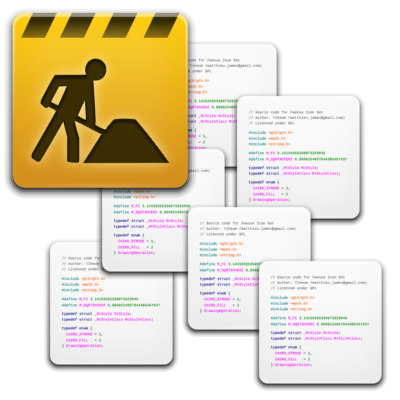
\includegraphics[width=1cm]{img/working_dir} & \textbf{répertoire de travail :} & \textbf{README (modifié)} \\
		
\includegraphics[width=1cm]{img/stash} & \textbf{fichiers indexés :} & vide\\
		
\includegraphics[width=1cm]{img/git_repo} & \textbf{dépôt local :} & commit \#1\\ 
		\end{tabular} 
	\end{center}
\end{frame}

\begin{frame}[fragile]{Constater les changements avec git status}
	\begin{lstlisting}[frame=single]
		git status
	\end{lstlisting}
	
	Les fichiers modifiés sont détectés; on propose de les indexer avec git add	
	
	\begin{figure}
		\centering
		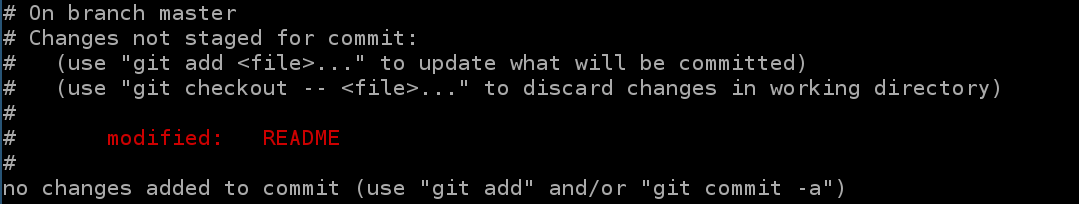
\includegraphics[width=11.5cm]{img/shot3}
	\end{figure}
\end{frame}

\begin{frame}[fragile]{Indexation du fichier modifié}
	\begin{lstlisting}[frame=single]
		git add README
	\end{lstlisting}
	
	\begin{center}
		\begin{tabular}{l c l}
		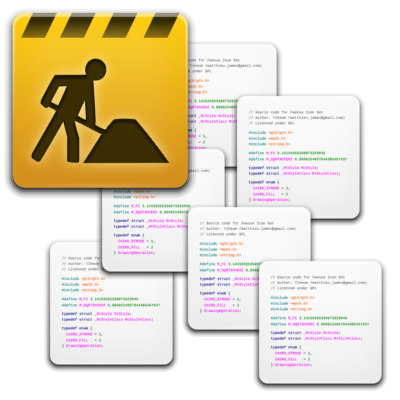
\includegraphics[width=1cm]{img/working_dir} & \textbf{répertoire de travail :} & README (modifié)\\
		
\includegraphics[width=1cm]{img/stash} & \textbf{fichiers indexés :} & \textbf{README (modifié)}\\
		
\includegraphics[width=1cm]{img/git_repo} & \textbf{dépôt local :} & commit \#1 {\tiny\textit{(Ajout du fichier README)}} \\ 
		\end{tabular} 
	\end{center}

	\begin{center}
		\textit{(vérifier avec git status)}
	\end{center}
\end{frame}

\begin{frame}[fragile]{Validation des changements}
	\begin{lstlisting}[frame=single]
		git commit -m "Modification du fichier README"
	\end{lstlisting}
	
	\begin{center}
		\begin{tabular}{l c l}
		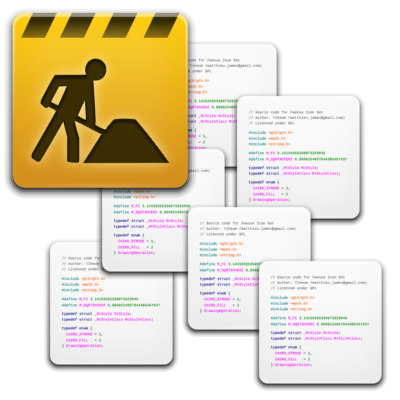
\includegraphics[width=1cm]{img/working_dir} & \textbf{répertoire de travail :} & README (modifié)\\
		
\includegraphics[width=1cm]{img/stash} & \textbf{fichiers indexés :} & \textbf{vide}\\
		
\includegraphics[width=1cm]{img/git_repo} & \textbf{dépôt local :} & commit \#1, \textbf{commit \#2}\\
		\end{tabular} 
	\end{center}

	\begin{center}
		\textit{(vérifier avec git status)}
	\end{center}
\end{frame}

\begin{frame}{Historique des commits}

	\begin{figure}
		\centering
		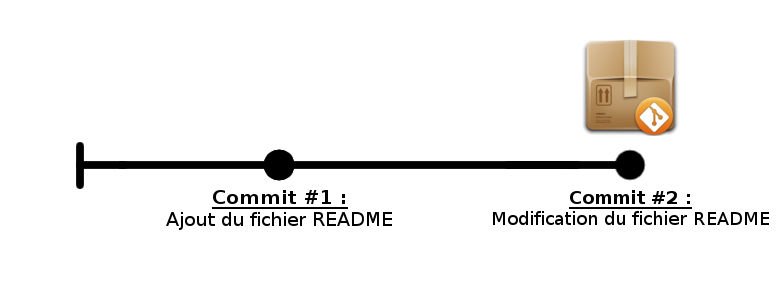
\includegraphics[width=11cm]{img/repo3}
	\end{figure}
\end{frame}

\begin{frame}[fragile]{Historique des commits}
	\begin{lstlisting}[frame=single]
		git log
	\end{lstlisting}
		
	\begin{figure}
		\centering
		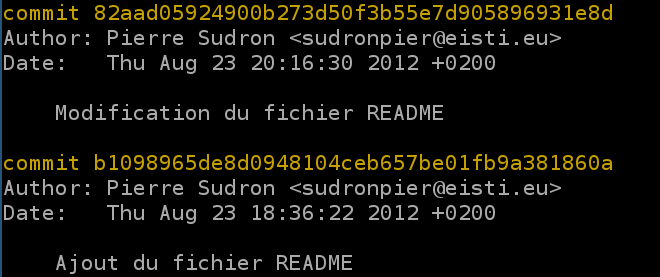
\includegraphics[width=11.5cm]{img/shot4}
	\end{figure}
\end{frame}

\begin{frame}{Export vers un dépôt git en ligne}
	Nous utiliserons une instance \textbf{GitLab} disponible à l'adresse :
	\begin{center}
	\url{http://gitlab-test.ccr.eisti.fr/}
	\end{center}
	\begin{figure}
  		\centering
 		
\includegraphics[height=1cm]{img/gitlab-logo}
	\end{figure}
	
	Il existe de nombreux sites permettant d'héberger vos projets git, dont :
	\begin{itemize}
		\item GitHub
		\item Gitorious
	\end{itemize}
\end{frame}

\begin{frame}{Se connecter et ajuster son profil sur GitLab}
	\begin{figure}
  		\centering
 		\includegraphics[height=6cm]{img/shot10}
	\end{figure}
\end{frame}

\begin{frame}{Créer un projet sur GitLab}
	(mettre des captures d'écran)
\end{frame}

\begin{frame}[fragile]{Créer une clé SSH}
	Ouvrez un nouveau terminal :
	\begin{lstlisting}[frame=single]
		ssh-keygen -t rsa -C "email@troll.com"
	\end{lstlisting}
	
	La clé SSH permet :
	\begin{itemize}
		\item de vous identifier formellement
		\item de crypter de transfert de code entre vous et le serveur
	\end{itemize}
	\begin{figure}
  		\centering
 		\includegraphics[height=2.5cm]{img/keyhole}
	\end{figure}
\end{frame}

\begin{frame}[fragile]{Indiquer la clé publique à GitLab}
	Le RSA est un cryptage asymétrique, et créé un jeu de deux clés
	\begin{itemize}
		\item une clé privée
		\item une \textbf{clé publique}
	\end{itemize}
	
	Pour afficher la clé publique :
	\begin{lstlisting}[frame=single]
		cat .ssh/id_rsa.pub
	\end{lstlisting}
	\begin{itemize}
		\item ajouter la clé publique au trousseau GitLab
	\end{itemize}		
	\begin{center}
		\textit{(vous pouvez fermer le second terminal et revenir au précédent)}
	\end{center}
\end{frame}

\begin{frame}[fragile]{Ajouter le dépôt dans votre projet}
	\begin{lstlisting}[frame=single]
		git remote add origin
	\end{lstlisting}
	
	\begin{itemize}
		\item \textbf{origin :} nom donné au serveur distant par convention
	\end{itemize}
\end{frame}

\begin{frame}[fragile]{Mettre le projet en ligne !}
	\begin{lstlisting}[frame=single]
		git push -u origin master
	\end{lstlisting}
	
	\begin{itemize}
		\item \textbf{origin :} nom donné au serveur distant par convention
		\item \textbf{master :} nom donné au dépôt local par défaut
	\end{itemize}
	
	\begin{figure}
  		\centering
 		\subfloat{\includegraphics[height=2.5cm]{img/git_repo}}     
		\subfloat{\includegraphics[height=1.5cm]{img/forward}}
  		\subfloat{\includegraphics[height=2.5cm]{img/web}}
	\end{figure}
	\begin{center}
		\begin{tabular}{p{3.5cm}  p{1cm} p{2cm}}
		\centering master & & origin
		\end{tabular}
	\end{center}
\end{frame}

\begin{frame}{Voir le résultat sur GitLab}
	Il ne reste plus qu'à constater le résultat avec satisfaction !
	(mettre des captures d'écran)
\end{frame}


\begin{frame}
	\begin{center}
		{\small  \textit{avant de continuer...}}\\
 		\Large{la Pause !} 		
	\end{center}

	\begin{figure}
		\centering
		\includegraphics[height=3cm]{img/cafe}
	\end{figure}
\end{frame}


\begin{frame}
	\begin{center}
 		\Large{Partie 2 : Travailler à plusieurs}\\
 		{\small  \textit{découverte des fonctionnalités de partage}}
	\end{center}

	\begin{figure}
		\centering
		\includegraphics[height=3cm]{img/web}
	\end{figure}
\end{frame}

\begin{frame}
	Partie pas faite... En gros, on reprend les concepts données plus haut, mais sur un projet à plusieurs.
\end{frame}

\begin{frame}
	\begin{center}
 		\Large{Partie 3 : Comment ça va vieille branche ?}\\
 		{\small  \textit{développer en parallèle}}
	\end{center}

	\begin{figure}
		\centering
		\includegraphics[height=3cm]{img/web}
	\end{figure}
\end{frame}

\begin{frame}{De quoi ai-je besoin ?}
	\begin{center}
 		\Large{logiciel Meld}\\
	\end{center}

	\begin{figure}
		\centering
		\includegraphics[height=3cm]{img/meld}
	\end{figure}
\end{frame}

\begin{frame}{C'est l'histoire d'un prof...}
	Jean-Paul a fini de rédiger le poly du cours de cette année, en \LaTeX{} bien entendu !\\
	
	
	Il souhaite continuer à rajouter des parties pour l'anné suivante tout en gardant une version de cette année afin de corriger les coquilles que ses élèves lui signalent.\\
	Mais comme Jean Paul n'est pas très organisé, nous allons l'aider à mieux gérer son texte de cours avec \textbf{git} et les \textbf{branches} !	
\end{frame}

\begin{frame}{Le principe des branches}
	Fourche dans le processus de développement du projet. Une branche démarre à partir d'un commit donné.
	
	\begin{figure}
		\centering
		\includegraphics[width=11cm]{img/repo4}
	\end{figure}
\end{frame}

\begin{frame}{Le principe des branches}
	Nous allons créer une branche dédiée aux corrections des fautes d'orthographe sur une branche partant de la version distribuée du poly.
	
	\begin{figure}
		\centering
		\includegraphics[width=11cm]{img/repo4-2}
	\end{figure}
\end{frame}

\begin{frame}[fragile]{Préparation du projet}
	\begin{itemize}
		\item créer un dossier \texttt{formation\_git\_branches}
		\item déplacer le fichier \texttt{cours.tex} fourni dans ce dossier
	\end{itemize}
	
	\begin{lstlisting}[frame=single]
		cd formation_git_branches
	\end{lstlisting}
	\begin{lstlisting}[frame=single]
		git init
	\end{lstlisting}
	\begin{lstlisting}[frame=single]
		git git add cours.tex
	\end{lstlisting}
	\begin{lstlisting}[frame=single]
		git commit -m "Version rentree"
	\end{lstlisting}
\end{frame}

\begin{frame}[fragile]{Créer une branche}
	La branche est créée à partir du dernier commit local (HEAD).
	\begin{lstlisting}[frame=single]
		git branch rentree_suivante
	\end{lstlisting}
	
	\vfill{}
	Pour lister les branches existantes : 

	\begin{lstlisting}[frame=single]
		git branch
	\end{lstlisting}
	\begin{figure}
		\centering
		\includegraphics[height=1cm]{img/shot5}
	\end{figure}
\end{frame}

\begin{frame}[fragile]{Sauter de branche en branche}
	
	\begin{lstlisting}[frame=single]
		git checkout rentree_suivante
	\end{lstlisting}
	
	\vfill{}
	La commande git branch donne le résultat suivant :

	\begin{figure}
		\centering
		\includegraphics[height=1cm]{img/shot6}
	\end{figure}
\end{frame}

\begin{frame}[fragile]{Ajouter un nouveau paragraphe pour la rentrée prochaine}

	Jean-Paul, studieux comme toujours, ne tarde pas à rajouter du contenu pour l'année prochaine.
	\vfill{}
	Éditer le fichier \texttt{cours.tex} en ajoutant une ligne à la fin. Sauvegarder, fermer l'éditeur de texte et commiter.	
	
	\begin{lstlisting}[frame=single]
		git add cours.tex
		git commit -m "Nouveau paragraphe"
	\end{lstlisting}
	
\end{frame}

\begin{frame}[fragile]{Revenir sur la branche principale pour une correction}

	Mince ! On a signalé la présence de fautes d'orthographe dans le poly de cette année.
	\vfill{}
	Retourner sur la branche principale	
	
	\begin{lstlisting}[frame=single]
		git checkout master
	\end{lstlisting}
	
	Ouvrir le fichier \texttt{cours.tex} avec un éditeur. Vérifier qu'il s'agit bien de la version de cette rentrée.\\
	Corriger les fautes, enregistrer, commiter.
	
\end{frame}

\begin{frame}[fragile]{Visualiser les commits selon leur branche}

	\begin{lstlisting}[frame=single]
		git log --oneline --graph --all
	\end{lstlisting}
	
	\begin{figure}
		\centering
		\includegraphics[width=11cm]{img/shot7}
	\end{figure}
	\begin{center}
	\textit{le log se lit de bas en haut}
	\end{center}
\end{frame}

\begin{frame}{Fusionner deux branches}

	La rentrée suivante est arrivée (ça passe vite), et Jean-Paul voudrait intégrer ses nouvelles parties tout en conservant les corrections faites en cours d'année. 
	\begin{figure}
		\centering
		\includegraphics[width=11cm]{img/repo5}
	\end{figure}
\end{frame}

\begin{frame}[fragile]{Fusionner deux branches}
	Se placer dans la branche qui va "intégrer" les commits de l'autre
	\begin{lstlisting}[frame=single]
		git checkout master
	\end{lstlisting}
	
	Réaliser la fusion
	\begin{lstlisting}[frame=single]
		git merge rentree_suivante
	\end{lstlisting}
	
	... et là : \textbf{Merge conflict} !
	\begin{figure}
		\centering
		\includegraphics[width=11cm]{img/shot8}
	\end{figure}
	Certains paragraphes ont un contenu différent, il va falloir gérer ça à la main.
\end{frame}

\begin{frame}[fragile]{Gérer un merge conflict}
	Ouvrir le fichier \texttt{cours.tex}. git a modifié son contenu pour mettre en évidence le conflit.
	\begin{lstlisting}[frame=single]
		<<<<<<< HEAD
		    ancien contenu
		=======
		    nouveau contenu
		>>>>>>> rentree_suivante
	\end{lstlisting}
	
	git status permet de voir sur quels fichiers il existe des conflits :
	\begin{figure}
		\centering
		\includegraphics[width=11cm]{img/shot9}
	\end{figure}
\end{frame}

\begin{frame}[fragile]{Gérer un merge conflict}
	La démarche à suivre pour résoudre le conflit :
	\begin{itemize}
		\item corriger les conflits dans chaque fichier concerné
		\item vérifier que tous les conflits sont corrigés avec \textbf{git status}
		\item indexer (\textbf{git add}) tous les fichiers modifiés dans la manipulation
		\item commiter (\textbf{git commit}), on appelle ça un \textit{'merge commit'}
	\end{itemize}
\end{frame}

\begin{frame}[fragile]{Corriger des conflits dans un fichier plus facilement}
	Il est assez compliqué de s'en sortir avec ça :
	\begin{lstlisting}[frame=single]
		<<<<<<< HEAD
		    ancien contenu
		=======
		    nouveau contenu
		>>>>>>> rentree_suivante
	\end{lstlisting}
	
	On va utiliser un outil graphique : \textbf{Meld} (il existe énormément d'équivalents)
	\begin{figure}
		\centering
		\includegraphics[height=2cm]{img/meld}
	\end{figure}
\end{frame}

\begin{frame}[fragile]{Corriger des conflits dans un fichier plus facilement}
	
	\begin{lstlisting}[frame=single]
		git mergetool
	\end{lstlisting}
	mergetool va lancer Meld (ou équivalent) pour chaque fichier où il y a un conflit.
	\begin{figure}
		\centering
		\includegraphics[height=2cm]{img/meld}
	\end{figure}
\end{frame}

\begin{frame}{Utiliser Meld}
	Meld (et équivalents) présente sur trois colonnes, trois version du fichier :
	\begin{itemize}
		\item \textbf{locale} à gauche : votre dernière version de la branche réceptrice
		\item \textbf{remote} à droite : la dernière version de la branche à fusionner
		\item \textbf{origin} au centre : la dernière version commune aux deux branches
	\end{itemize}
	
	Dans la pratique, on enregistrera le résultat voulu dans la colonne centrale, c'est à dire sur \textbf{origin}.
\end{frame}

\begin{frame}[fragile]{Finaliser la résolution de conflits}

	mergetool créé un fichier de sauvegarde \texttt{<fichier>.orig}, on peut les supprimer une fois la session mergetool terminée
	\vfill{}
	
	Il faut faire un \textit{merge commit} : valider la résolution des conflits au sein d'un commit
	\begin{lstlisting}[frame=single]
		git status
		git add cours.tex
		git commit -m "Merge dans master de rentree_suivante"
	\end{lstlisting}	
\end{frame}

\begin{frame}[fragile]{Terminer une branche}

	\begin{lstlisting}[frame=single]
		git branch -d rentree_suivante
	\end{lstlisting}
	\vfill{}
	Il possible de terminer seulement une branche qui a été merge.
	Pour forcer la suppression d'une branche :
	\begin{lstlisting}[frame=single]
		git branch -D rentree_suivante
	\end{lstlisting}
	
\end{frame}

\begin{frame}
	\begin{center}
 		\Large{Bonus : Quelques conseils}\\
 		{\small  \textit{tout va bien se passer...}}
	\end{center}

	\begin{figure}
		\centering
		\includegraphics[height=3cm]{img/bonus}
	\end{figure}
\end{frame}

\begin{frame}{Commitez bien, commitez souvent}

	\begin{itemize}
		\item segmentez les tâches, faites un commit dès que possible
		\item testez votre code avant de faire un commit
	\end{itemize}
	
\end{frame}

\begin{frame}{Les branches c'est bon, mangez-en !}
	\begin{figure}
		\centering
		\includegraphics[height=4cm]{img/koala-eating-leaf}
	\end{figure}

	\begin{itemize}
		\item séparez les tâches indépendantes
		\item n'hésitez pas à faire des expérimentations dans une branche dédiée
	\end{itemize}
	
\end{frame}

\begin{frame}{Jouez collectif}

	\begin{itemize}
		\item organisez-vous et concertez-vous avec vos partenaires
		\item suivez les avancées des autres, donnez votre avis
	\end{itemize}
	
\end{frame}

% ----------------

\begin{frame}
		\begin{center}
 		\Large{Des questions ?}\\
 		{\small \textit{Ne mourrons pas idiots.}}
	\end{center}

	\begin{figure}
		\centering
		\includegraphics[height=3cm]{img/help}
	\end{figure}
\end{frame}


\begin{frame}
		\begin{center}
 		\Large{Merci de votre participation}\\
 		{\small \textit{et à une prochaine fois !}}
	\end{center}

	\begin{figure}
		\centering
		\includegraphics[height=3cm]{img/git_repo}
	\end{figure}
\end{frame}


\end{document}

